% Source: TeX Live PGF manual, positioning library base-anchor example.
\documentclass[border=2pt]{standalone}
\usepackage{tikz}
\usetikzlibrary{positioning}

\begin{document}
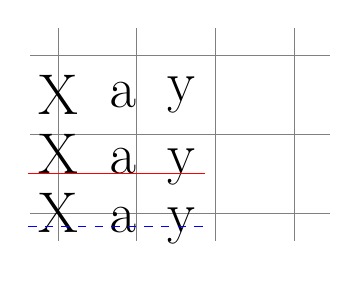
\begin{tikzpicture}[node distance=1ex, font=\huge]
  \draw[help lines] (-0.35,-0.35) grid (3.45,2.35);

  \node (right-X) at (0,1.5) {X};
  \node (right-a) [right=of right-X] {a};
  \node (right-y) [right=of right-a] {y};

  \node (base-X) at (0,0.75) {X};
  \node (base-a) [base right=of base-X] {a};
  \node (base-y) [base right=of base-a] {y};
  \draw[red,thin] (base-X.base west) -- (base-y.base east);

  \node (mid-X) at (0,0) {X};
  \node (mid-a) [mid right=of mid-X] {a};
  \node (mid-y) [mid right=of mid-a] {y};
  \draw[blue,thin,dashed] (mid-X.mid west) -- (mid-y.mid east);
\end{tikzpicture}
\end{document}
